\documentclass[11pt,a4paper]{article}
\usepackage[utf8]{inputenc}
\usepackage[margin=1in]{geometry}
\usepackage{hyperref}
\usepackage{booktabs}
\usepackage{tikz}
\usetikzlibrary{shapes.geometric, arrows, positioning}
\usepackage{float}
\usepackage{enumitem}

% Configure hyperlinks
\hypersetup{
    colorlinks=true,
    linkcolor=blue,
    urlcolor=cyan,
}

\title{\textbf{TradeSymphony} \\ 
       \large Multi-Agent Investment Analysis System}
\date{\today}

\begin{document}

\maketitle

\begin{abstract}
TradeSymphony is a multi-agent AI system built on CrewAI that replicates the collaborative decision-making structure of institutional investment firms. The system employs specialized AI agents working in a hierarchical organization to perform comprehensive investment analysis and generate portfolio recommendations. This document provides a concise overview of the system architecture, agent design, and multi-agent coordination mechanisms.
\end{abstract}

\section{System Overview}

\subsection{Problem Domain}
Investment analysis requires diverse expertise spanning fundamental analysis, risk assessment, compliance monitoring, and strategic decision-making. Traditional approaches suffer from human biases and scalability limitations.

\subsection{Solution Approach}
TradeSymphony addresses these challenges through a multi-agent architecture where specialized AI agents collaborate within a structured organizational framework, mimicking institutional investment firms while leveraging AI consistency and computational power.

\section{Multi-Agent Architecture}

\subsection{Agent Hierarchy}

The system implements a professional investment firm structure with 10 specialized agents:

\begin{figure}[H]
\centering
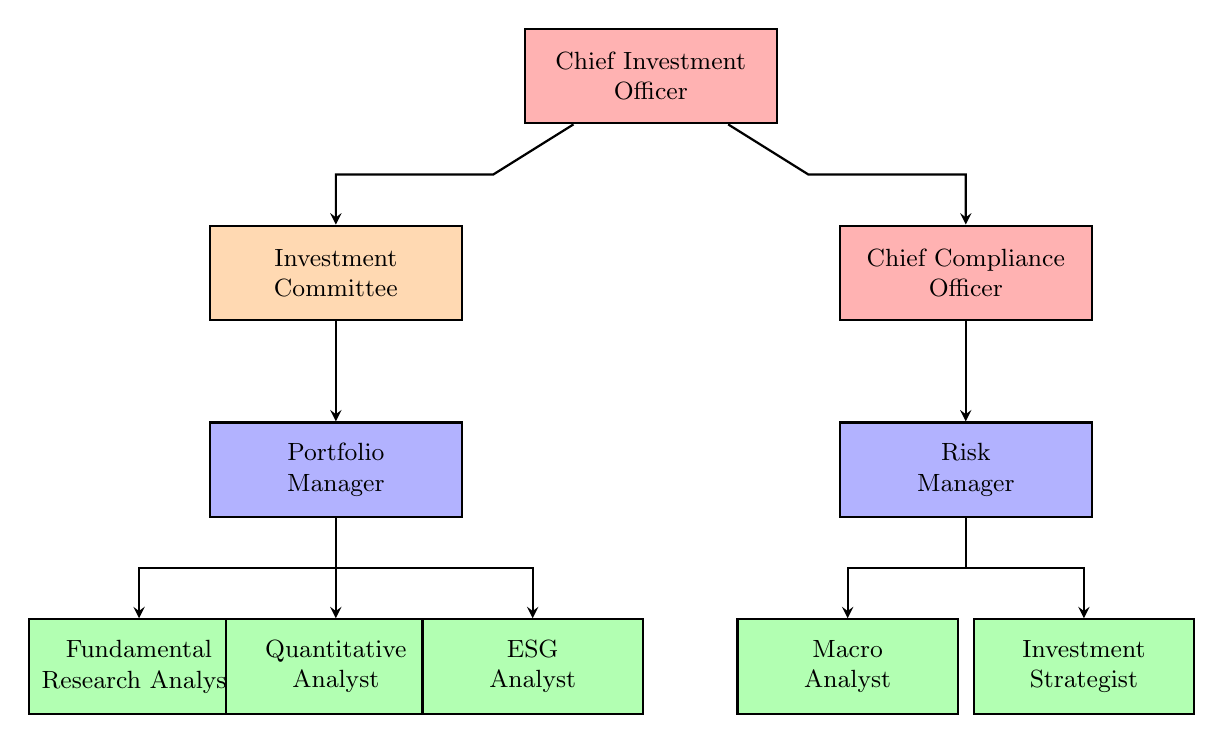
\begin{tikzpicture}[
    % Styles for each node type
    executive/.style={rectangle, draw=black, thick, align=center, fill=red!30, minimum width=3.2cm, minimum height=1.2cm, font=\small},
    committee/.style={rectangle, draw=black, thick, align=center, fill=orange!30, minimum width=3.2cm, minimum height=1.2cm, font=\small},
    management/.style={rectangle, draw=black, thick, align=center, fill=blue!30, minimum width=3.2cm, minimum height=1.2cm, font=\small},
    analyst/.style={rectangle, draw=black, thick, align=center, fill=green!30, minimum width=2.8cm, minimum height=1.2cm, font=\small},
    arrow/.style={thick, ->, >=stealth, black}
]

% Top Executive (Level 1)
\node[executive] (cio) at (0,0) {Chief Investment\\Officer};

% Second Tier (Level 2) - properly spaced
\node[committee]  (ic)  at (-4,-2.5) {Investment\\Committee};
\node[executive]  (cco) at (4,-2.5) {Chief Compliance\\Officer};

% Third Tier (Level 3) - aligned under their supervisors
\node[management] (pm) at (-4,-5) {Portfolio\\Manager};
\node[management] (rm) at (4,-5) {Risk\\Manager};

% Fourth Tier (Level 4) - properly distributed under Portfolio Manager
\node[analyst] (fra) at (-6.5,-7.5) {Fundamental\\Research Analyst};
\node[analyst] (qa)  at (-4,-7.5) {Quantitative\\Analyst};
\node[analyst] (esg) at (-1.5,-7.5) {ESG\\Analyst};

% Fourth Tier under Risk Manager - properly distributed
\node[analyst] (ma)  at (2.5,-7.5) {Macro\\Analyst};
\node[analyst] (is)  at (5.5,-7.5) {Investment\\Strategist};

% Draw connecting arrows with proper hierarchy
% CIO to second tier
\draw[arrow] (cio) -- (-2,-1.25) -- (-4,-1.25) -- (ic);
\draw[arrow] (cio) -- (2,-1.25) -- (4,-1.25) -- (cco);

% Second tier to third tier
\draw[arrow] (ic) -- (pm);
\draw[arrow] (cco) -- (rm);

% Third tier to fourth tier - Portfolio Manager branch
\draw[arrow] (pm) -- (-4,-6.25) -- (-6.5,-6.25) -- (fra);
\draw[arrow] (pm) -- (qa);
\draw[arrow] (pm) -- (-4,-6.25) -- (-1.5,-6.25) -- (esg);

% Third tier to fourth tier - Risk Manager branch
\draw[arrow] (rm) -- (4,-6.25) -- (2.5,-6.25) -- (ma);
\draw[arrow] (rm) -- (4,-6.25) -- (5.5,-6.25) -- (is);

\end{tikzpicture}
\caption{TradeSymphony Agent Organizational Structure}
\end{figure}

\subsection{Core Agent Roles}

\begin{table}[H]
\centering
\small
\begin{tabular}{@{}p{3cm}p{4cm}p{4.5cm}@{}}
\toprule
\textbf{Agent} & \textbf{Primary Function} & \textbf{Key Tools} \\
\midrule
Chief Investment Officer & Final investment decisions \& strategy oversight & Portfolio Optimization, Macro Analysis, Risk Assessment \\
\midrule
Investment Committee & Collective review \& voting on recommendations & Risk Assessment, Portfolio Optimization, Compliance \\
\midrule
Chief Compliance Officer & Regulatory compliance \& risk oversight & Compliance Check, Tavily Search, Firecrawl Research \\
\midrule
Portfolio Manager & Portfolio construction \& execution & Portfolio Optimization, Stock Screener, Technical Analysis \\
\midrule
Risk Manager & Risk assessment \& mitigation & Risk Assessment, Market Simulation, Macro Analysis \\
\midrule
Fundamental Research Analyst & Company \& industry analysis & Financial Data, Company Research, Alpha Vantage \\
\midrule
Quantitative Analyst & Statistical modeling \& screening & Stock Screener, Technical Analysis, Financial Analysis \\
\midrule
ESG Analyst & Environmental, social \& governance evaluation & Company Research, Sentiment Analysis, Firecrawl \\
\midrule
Macro Analyst & Economic trends \& market outlook & Macro Analysis, Financial Data, Sentiment Analysis \\
\midrule
Investment Strategist & Strategy development \& communication & Portfolio Optimization, Stock Screener, Macro Analysis \\
\bottomrule
\end{tabular}
\caption{Agent Roles and Tool Ecosystem}
\end{table}

\section{System Architecture}

\subsection{Technology Stack}

\begin{itemize}
    \item \textbf{Framework}: CrewAI for multi-agent orchestration with sequential processing
    \item \textbf{Memory Architecture}: 
    \begin{itemize}
        \item Long-term: LTMSQLiteStorage (persistent learning)
        \item Short-term: RAGStorage with OpenAI embeddings (session context)
        \item Entity: Vector storage with ChromaDB (company knowledge)
    \end{itemize}
    \item \textbf{Tool Ecosystem}: 19 specialized financial analysis tools
    \item \textbf{Data Sources}: Yahoo Finance, Alpha Vantage, Tavily Search, Firecrawl
    \item \textbf{LLM Integration}: OpenAI GPT-4o-mini with temperature control
    \item \textbf{Monitoring}: LangSmith integration for workflow tracking
\end{itemize}

\subsection{Workflow Process}

The system executes a sequential 10-task workflow replicating institutional investment processes:

\begin{figure}[H]
\centering
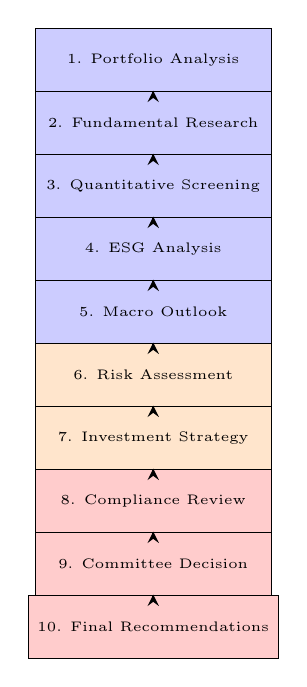
\begin{tikzpicture}[node distance=0.8cm, auto]
    \tikzstyle{analysis}   = [rectangle, minimum width=3.0cm, minimum height=0.8cm, text centered, draw=black, fill=blue!20, font=\tiny]
    \tikzstyle{synthesis}  = [rectangle, minimum width=3.0cm, minimum height=0.8cm, text centered, draw=black, fill=orange!20, font=\tiny]
    \tikzstyle{decision}   = [rectangle, minimum width=3.0cm, minimum height=0.8cm, text centered, draw=black, fill=red!20, font=\tiny]
    \tikzstyle{arrow}      = [thick,->,>=stealth]
    
    % Analysis Phase
    \node [analysis] (portfolio)    {1. Portfolio Analysis};
    \node [analysis, below of=portfolio]    (fundamental) {2. Fundamental Research};
    \node [analysis, below of=fundamental]  (quant)      {3. Quantitative Screening};
    \node [analysis, below of=quant]        (esg)        {4. ESG Analysis};
    \node [analysis, below of=esg]          (macro)      {5. Macro Outlook};
    
    % Risk Assessment
    \node [synthesis, below of=macro]       (risk)       {6. Risk Assessment};
    
    % Strategy Development
    \node [synthesis, below of=risk]        (strategy)   {7. Investment Strategy};
    
    % Governance
    \node [decision, below of=strategy]     (compliance) {8. Compliance Review};
    \node [decision, below of=compliance]   (committee)  {9. Committee Decision};
    \node [decision, below of=committee]    (final)      {10. Final Recommendations};
    
    % Arrows
    \draw [arrow] (portfolio)   -- (fundamental);
    \draw [arrow] (fundamental) -- (quant);
    \draw [arrow] (quant)       -- (esg);
    \draw [arrow] (esg)         -- (macro);
    \draw [arrow] (macro)       -- (risk);
    \draw [arrow] (risk)        -- (strategy);
    \draw [arrow] (strategy)    -- (compliance);
    \draw [arrow] (compliance)  -- (committee);
    \draw [arrow] (committee)   -- (final);
    
\end{tikzpicture}
\caption{Sequential Investment Analysis Workflow}
\end{figure}

\subsection{Key Features}

\begin{itemize}[itemsep=0.5em]
    \item \textbf{Collaborative Intelligence}: Agents share insights and build consensus
    \item \textbf{Hierarchical Decision-Making}: Senior agents validate junior agent analyses
    \item \textbf{Memory Persistence}: System learns from previous analyses
    \item \textbf{Tool Integration}: Specialized tools for each analysis domain
    \item \textbf{Scalable Processing}: Handles multiple portfolios simultaneously
\end{itemize}

\section{Implementation Details}

\subsection{Agent Communication}
Agents communicate through CrewAI's sequential task execution model with context sharing:
\begin{itemize}
    \item Sequential task execution with context dependency chains
    \item Memory-based knowledge sharing across the workflow
    \item Hierarchical validation through committee and executive review
    \item LangSmith monitoring for workflow transparency and debugging
\end{itemize}

\subsection{Memory Architecture}
The three-tier memory system provides persistent learning and context retention:
\begin{itemize}
    \item \textbf{Long-term}: LTMSQLiteStorage for historical patterns and decision learning
    \item \textbf{Short-term}: RAGStorage with OpenAI embeddings for session context
    \item \textbf{Entity}: Vector storage using ChromaDB for company-specific knowledge
\end{itemize}

\subsection{Task-Agent Mapping}
The 10-task workflow is distributed across specialized agents as follows:
\begin{itemize}
    \item \textbf{Portfolio Manager}: Portfolio Analysis (Task 1)
    \item \textbf{Fundamental Research Analyst}: Fundamental Research (Task 2)
    \item \textbf{Quantitative Analyst}: Quantitative Screening (Task 3)
    \item \textbf{ESG Analyst}: ESG Analysis (Task 4)
    \item \textbf{Macro Analyst}: Macro Outlook (Task 5)
    \item \textbf{Risk Manager}: Risk Assessment (Task 6)
    \item \textbf{Investment Strategist}: Investment Strategy (Task 7)
    \item \textbf{Chief Compliance Officer}: Compliance Review (Task 8)
    \item \textbf{Investment Committee}: Committee Decision (Task 9)
    \item \textbf{Chief Investment Officer}: Final Recommendations (Task 10)
\end{itemize}

\subsection{Tool Ecosystem}
The system provides 19 specialized financial analysis tools distributed across agent domains:
\begin{itemize}
    \item \textbf{Data Sources}: Yahoo Finance Tool, Alpha Vantage Tool, Financial Data Tool
    \item \textbf{Research Tools}: Tavily Search, Firecrawl Research, Company Research, Browser Research
    \item \textbf{Analysis Tools}: Financial Analysis, Technical Analysis, Sentiment Analysis
    \item \textbf{Portfolio Tools}: Portfolio Optimization, Stock Screener, Stock Symbol Fetcher
    \item \textbf{Risk Tools}: Risk Assessment, Market Simulation
    \item \textbf{Specialized Tools}: Macroeconomic Analysis, Compliance Check, ESG Evaluation
\end{itemize}

\section{Research Applications}

\subsection{Multi-Agent Systems Research}
TradeSymphony provides a testbed for investigating:
\begin{itemize}
    \item Agent coordination and consensus mechanisms
    \item Hierarchical decision-making in AI systems
    \item Emergent behavior in collaborative AI
    \item Communication protocols for specialized agents
\end{itemize}

\subsection{Financial AI Research}
The platform enables research in:
\begin{itemize}
    \item AI-driven investment strategy development
    \item Collaborative financial decision-making
    \item Risk management through multi-agent systems
    \item Automated compliance and governance
\end{itemize}

\section{Limitations and Future Work}

\subsection{Current Limitations}
\begin{itemize}
    \item Dependency on external data APIs
    \item LLM knowledge cutoff limitations
    \item Computational complexity for large portfolios
    \item Limited real-time market data integration
\end{itemize}

\subsection{Future Enhancements}
\begin{itemize}
    \item Real-time streaming data integration
    \item Advanced machine learning model integration
    \item Multi-asset class support expansion
    \item Backtesting and strategy validation framework
\end{itemize}

\section{Conclusion}

TradeSymphony demonstrates the effective application of multi-agent systems to complex financial analysis tasks. The hierarchical agent architecture successfully replicates institutional decision-making processes while providing consistency and scalability advantages. The system serves as both a practical investment analysis tool and a research platform for advancing multi-agent AI applications in finance.

The modular design and extensive tool integration make it suitable for researchers investigating collaborative AI systems, while the financial domain expertise provides practical value for investment analysis applications.

\end{document}
